%\documentclass[
  bibliography=totoc,     % Literatur im Inhaltsverzeichnis
  captions=tableheading,  % Tabellenüberschriften
  titlepage=firstiscover, % Titelseite ist Deckblatt
]{scrartcl}

% Paket float verbessern
\usepackage{scrhack}

% Warnung, falls nochmal kompiliert werden muss
\usepackage[aux]{rerunfilecheck}

% unverzichtbare Mathe-Befehle
\usepackage{amsmath}
% viele Mathe-Symbole
\usepackage{amssymb}
% Erweiterungen für amsmath
\usepackage{mathtools}

% Fonteinstellungen
\usepackage{fontspec}
% Latin Modern Fonts werden automatisch geladen
% Alternativ zum Beispiel:
%\setromanfont{Libertinus Serif}
%\setsansfont{Libertinus Sans}
%\setmonofont{Libertinus Mono}

% Wenn man andere Schriftarten gesetzt hat,
% sollte man das Seiten-Layout neu berechnen lassen
\recalctypearea{}

% deutsche Spracheinstellungen
\usepackage[ngerman]{babel}


\usepackage[
  math-style=ISO,    % ┐
  bold-style=ISO,    % │
  sans-style=italic, % │ ISO-Standard folgen
  nabla=upright,     % │
  partial=upright,   % │
  mathrm=sym,        % ┘
  warnings-off={           % ┐
    mathtools-colon,       % │ unnötige Warnungen ausschalten
    mathtools-overbracket, % │
  },                       % ┘
]{unicode-math}

% traditionelle Fonts für Mathematik
\setmathfont{Latin Modern Math}
% Alternativ zum Beispiel:
%\setmathfont{Libertinus Math}

\setmathfont{XITS Math}[range={scr, bfscr}]
\setmathfont{XITS Math}[range={cal, bfcal}, StylisticSet=1]

% Zahlen und Einheiten
\usepackage[
  locale=DE,                   % deutsche Einstellungen
  separate-uncertainty=true,   % immer Unsicherheit mit \pm
  per-mode=symbol-or-fraction, % / in inline math, fraction in display math
]{siunitx}

% chemische Formeln
\usepackage[
  version=4,
  math-greek=default, % ┐ mit unicode-math zusammenarbeiten
  text-greek=default, % ┘
]{mhchem}

% richtige Anführungszeichen
\usepackage[autostyle]{csquotes}

% schöne Brüche im Text
\usepackage{xfrac}

% Standardplatzierung für Floats einstellen
\usepackage{float}
\floatplacement{figure}{htbp}
\floatplacement{table}{htbp}

% Floats innerhalb einer Section halten
\usepackage[
  section, % Floats innerhalb der Section halten
  below,   % unterhalb der Section aber auf der selben Seite ist ok
]{placeins}

% Seite drehen für breite Tabellen: landscape Umgebung
\usepackage{pdflscape}

% Captions schöner machen.
\usepackage[
  labelfont=bf,        % Tabelle x: Abbildung y: ist jetzt fett
  font=small,          % Schrift etwas kleiner als Dokument
  width=0.9\textwidth, % maximale Breite einer Caption schmaler
]{caption}
% subfigure, subtable, subref
\usepackage{subcaption}

% Grafiken können eingebunden werden
\usepackage{graphicx}

% schöne Tabellen
\usepackage{tabularray}
\UseTblrLibrary{booktabs, siunitx}

% Verbesserungen am Schriftbild
\usepackage{microtype}

% Literaturverzeichnis
\usepackage[
  backend=biber,
]{biblatex}
% Quellendatenbank
\addbibresource{lit.bib}
\addbibresource{programme.bib}

% Hyperlinks im Dokument
\usepackage[
  german,
  unicode,        % Unicode in PDF-Attributen erlauben
  pdfusetitle,    % Titel, Autoren und Datum als PDF-Attribute
  pdfcreator={},  % ┐ PDF-Attribute säubern
  pdfproducer={}, % ┘
]{hyperref}
% erweiterte Bookmarks im PDF
\usepackage{bookmark}

% Trennung von Wörtern mit Strichen
\usepackage[shortcuts]{extdash}

\author{%
  Vincent Wirsdörfer\\%
  \href{mailto:vincent.wirsdoerfer@udo.edu}{authorA@udo.edu}%
  \and%
  Joris Daus\\%
  \href{mailto:joris.daus@udo.edu}{authorB@udo.edu}%
}
\publishers{TU Dortmund – Fakultät Physik}


%\begin{document}
\section{Diskussion}
\label{sec:Diskussion}

Wie bereits in den vorherigen Kapiteln des Protokolls dargesetellt, werden diverse Untersuchungen der Ultraschallausbreitung 
in verschiedenen Materialen durchgeführt. Zu Beginn des Versuchs soll über die Geräte- und Programmeinstellung die Frequenz 
und Wellenlänge des Ultraschalls in Acryl berechnet. Wie dem Kapitel \ref{sec:Auswertung} zu entnehmen ist lauten die 
aufgenommen Werte wie folgt:

\begin{align*}
    f &= \sfrac{1}{T} = \qty{2}{\mega\hertz}\\
    \lambda &= c_\text{Acryl}\cdot{}f = \qty{1.831e-10}{\meter}
\end{align*}

\noindent Die Tatsache, dass bei allen fünf Messungen der Perdiodendauer ein Wert von $T = \qty{0.5}{\micro\second}$ gemssen 
wird, minimiert die Standardabweichung des Mittelwerts auf Null und begünstigt gleichermaßen die Präzision der Ergebnisse 
für die Wellenlänge und die Frequenz. Somit entspricht die empirisch bestimmte Frequenz exakt der Frequenz der verwendeten 
Sonde von $f = \qty{2}{\mega\hertz}$.\\

\noindent Im Anschluss werden die Schallgeschwindigkeiten in Aluminium und Acryl gemessen. Die dafür aufgenommenen Werte lauten 

\begin{align*}
    v_\text{Alu} &= \qty{6.46\pm0.08e3}{\meter\per\second} \\
    v_\text{Acryl} &= \qty{2.79\pm0.04e3}{\meter \per \second}.
\end{align*}

\noindent Diese Werte werden im Folgenden mit den recherchierten Literaturwerten

\begin{align*}
    c_\text{Aluminium} &= \qty{6320}{\meter \per \second}\\
    c_\text{Acryl}  &= \qty{2730}{\meter \per \second}
\end{align*}

\noindent abgeglichen. Wie zu erkennen ist, weicht der gemessene Mittelwert der Schallgeschwindigkeit von Aluminium um etwa \qty{2.22}{\percent}
vom Literaturwert ab. Bei Acryl beträgt die prozentuale Abweichung \qty{2.20}{\percent}. Beide Ergebnisse implizieren, dass 
keine signifikanten Fehler die Messung beeinträchtigen. Zusätzlich beschränkt sich die Versuchsdurchführung im Wesentlichen auf 
die Bedienung technischer Geräte, was den Eigenanteil an Fehlern minimiert und die Benennung potentieller Fehlerquellen
erschwert. Die trotzdem vorhandene Abweichung der Werte kann daher beispielsweise auf zu wenig Konktaktmittel zwischen Sonder 
und Zylinder oder auf mikroskopische Fehlerquellen im Zylinder hinweisen, welche ein ungewolltes Fehlerecho reflektieren 
und die Messwerte verfälschen. Zusätzlich könnte es sein, dass der Curser zur Bestimmung der Laufzeiten nicht vollständig den 
gewollten Zeitpeak trifft, sondern leicht daneben liegt, was leicht veränderte Schallgeschwindigkeiten der jeweiligen 
Materialien zur Folge hat.\\

\noindent Die Messung des Dämpfungskoeffizienten ist nur für Acryl möglich, da die Aluminiumzylinder bei wiederholten Messungen keinen 
exponentiellen Trend aufweisen und somit aus der Messung gestrichen werden! Für Acryl wird dagegen jedoch eine Dämpfungskurve 
mit der \qty{1}{\mega\hertz}- und mit der \qty{2}{\mega\hertz}-Sonde aufgenommen. Wie in der Auswertung bereits behandelt, bildet
die mit der \qty{2}{\mega\hertz}-Sonde tatsächlich, wie nach Gleichung \eqref{eqn:Intensitaet} postuliert, einen exponentiellen 
Abfall ab. Der Dämpfungskoeffizient in Acryl ist ein Parameter des \emph{curve\_fit} und lautet 

\begin{align*}
    \alpha_{\qty{2}{\mega\hertz}} = \qty{7.92\pm4.62}{\per\meter}
\end{align*}

\noindent Obwohl die gemessenen durch Werte durch eine abfallende Exponentialfunktion \emph{gefitted} werden können, ist die 
Aussagekräftigeit des Wertes aufgrund des großen Fehlers mit Vorsicht zu behandeln. Die hoher Fehleränfälligkeit des Parameters
ist durch starke Abweichung der Daten vom \emph{fit} zu erklären. Dies ist mittels Abbildung \ref{fig:Kurve2MHz} gut nachvollziehbar.
Systematisch betrachtet schlägt sich an dieser Stelle die Schwierigkeit wieder, speziell im Bereich kleiner Amplituden, dem 
Datenprogramm die korrekten Amplitudenwerte zu entnehmen. Dies wird aufgrund immer kleiner werdender und mehrerer Maxima erschwert.\\

\noindent Im Vergleich dazu gestaltet sich die Konstruktion des exponentiellen \emph{fits} bei der \qty{1}{\mega\hertz}-Sonde wesentlich 
schwieriger. Hierbei können keine Parameter ausgegeben werden, welche die Messdaten entsprechen \emph{fitten}. Die alternative Lösung des 
logarithmischen Ansatzes wird bereits in der Auswertung näher behandelt und liefert den Dämpfungskoeffizienten

\begin{align*}
    \alpha_{\qty{1}{\mega\hertz}} = \qty{31.19\pm7.15}{\per\meter}.
\end{align*}

\noindent Einerseits ist die Korrektheit dieses Wertes wegen der alternativen Methode nur schwer zu beurteilen. Andererseits 
ergibt die Erhöhung des Koeffizienten bei niedriger Frequenz der Sonder im Sachzusammenhang Sinn, da niedrigfrequente Wellen 
eine höhere Reichweite aufweisen.\\

\noindent Die Abbildung \ref{fig:Kalibrierkurve} zeigt, dass die Daten der Füllstandsmessung gut an einen \emph{polyfit} 2.
Ordnung gelegt werden können. Die zugehörigen der allgemeinen Funktionsgleichung

\begin{equation*}
    f(x) = ax² + bx + c
\end{equation*}

\noindent lauten wie folgt:

\begin{align*}
    a &= \qty{6.073\pm0.479e-4}{\micro\second\per\milli\liter\squared}\\  
    b &= \qty{0.107\pm0.012}{\micro\second\per\milli\liter}\\
    c &= \qty{10.71\pm0.698}{\micro\second }
\end{align*}

\noindent Der quadratische Zusammenhang kann in diesem Bereich der Messung insofern gerechtfertigt werden, da eine konstante 
Zugabe von Wasservolumen im letzten Bereich der Messung zu einer quadratischen Steigung der Höhe und somit auch der Laufzeit 
führt, was Resultat der besonderen Form des Erlenmeyerkolbens ist. 

\section{Anhang}

\begin{figure}
    \centering
    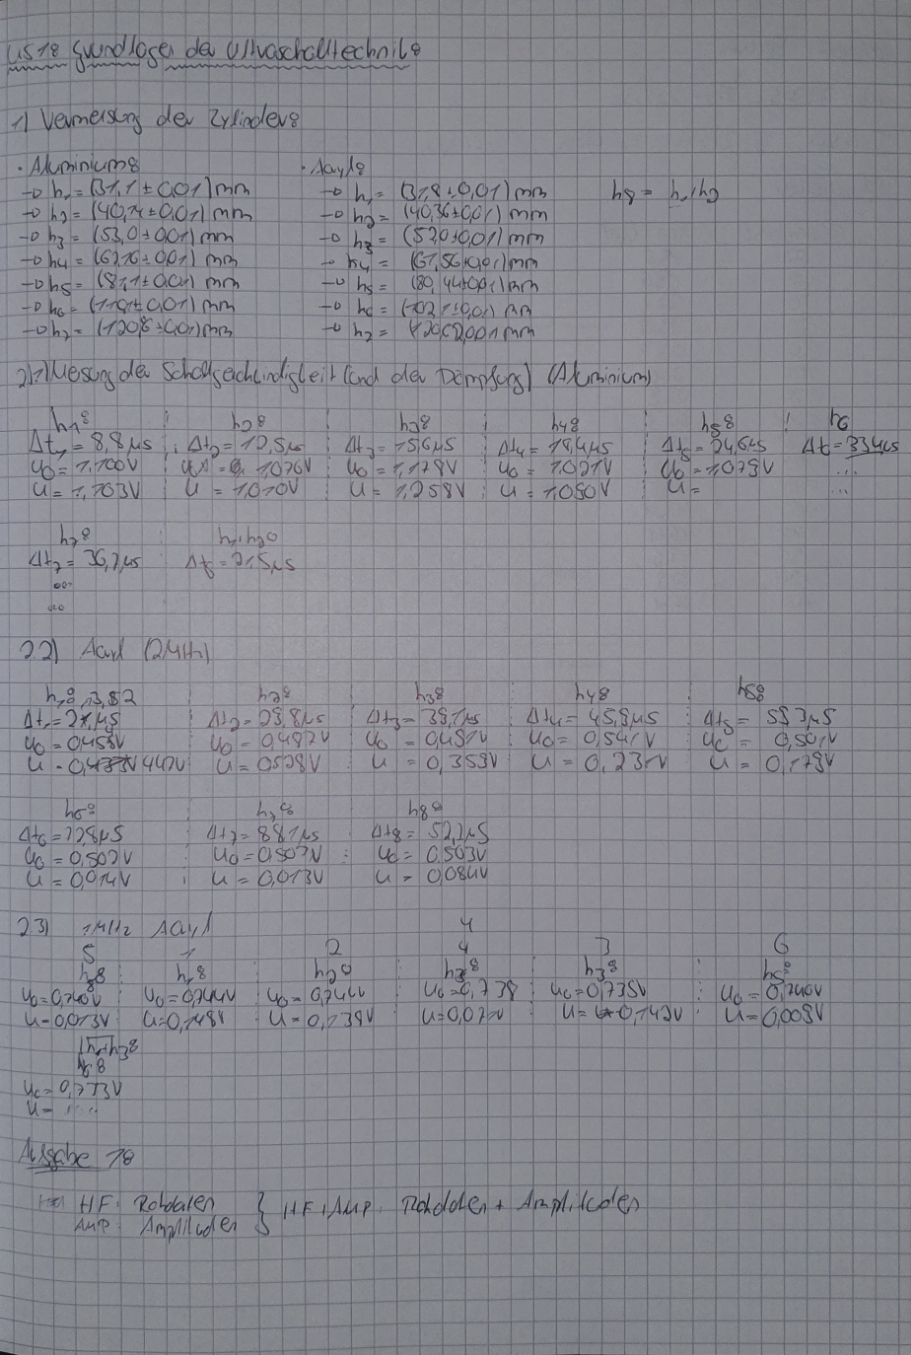
\includegraphics[width=0.9\textwidth]{Laborbuch1.jpg}
\end{figure}

\begin{figure}
    \centering
    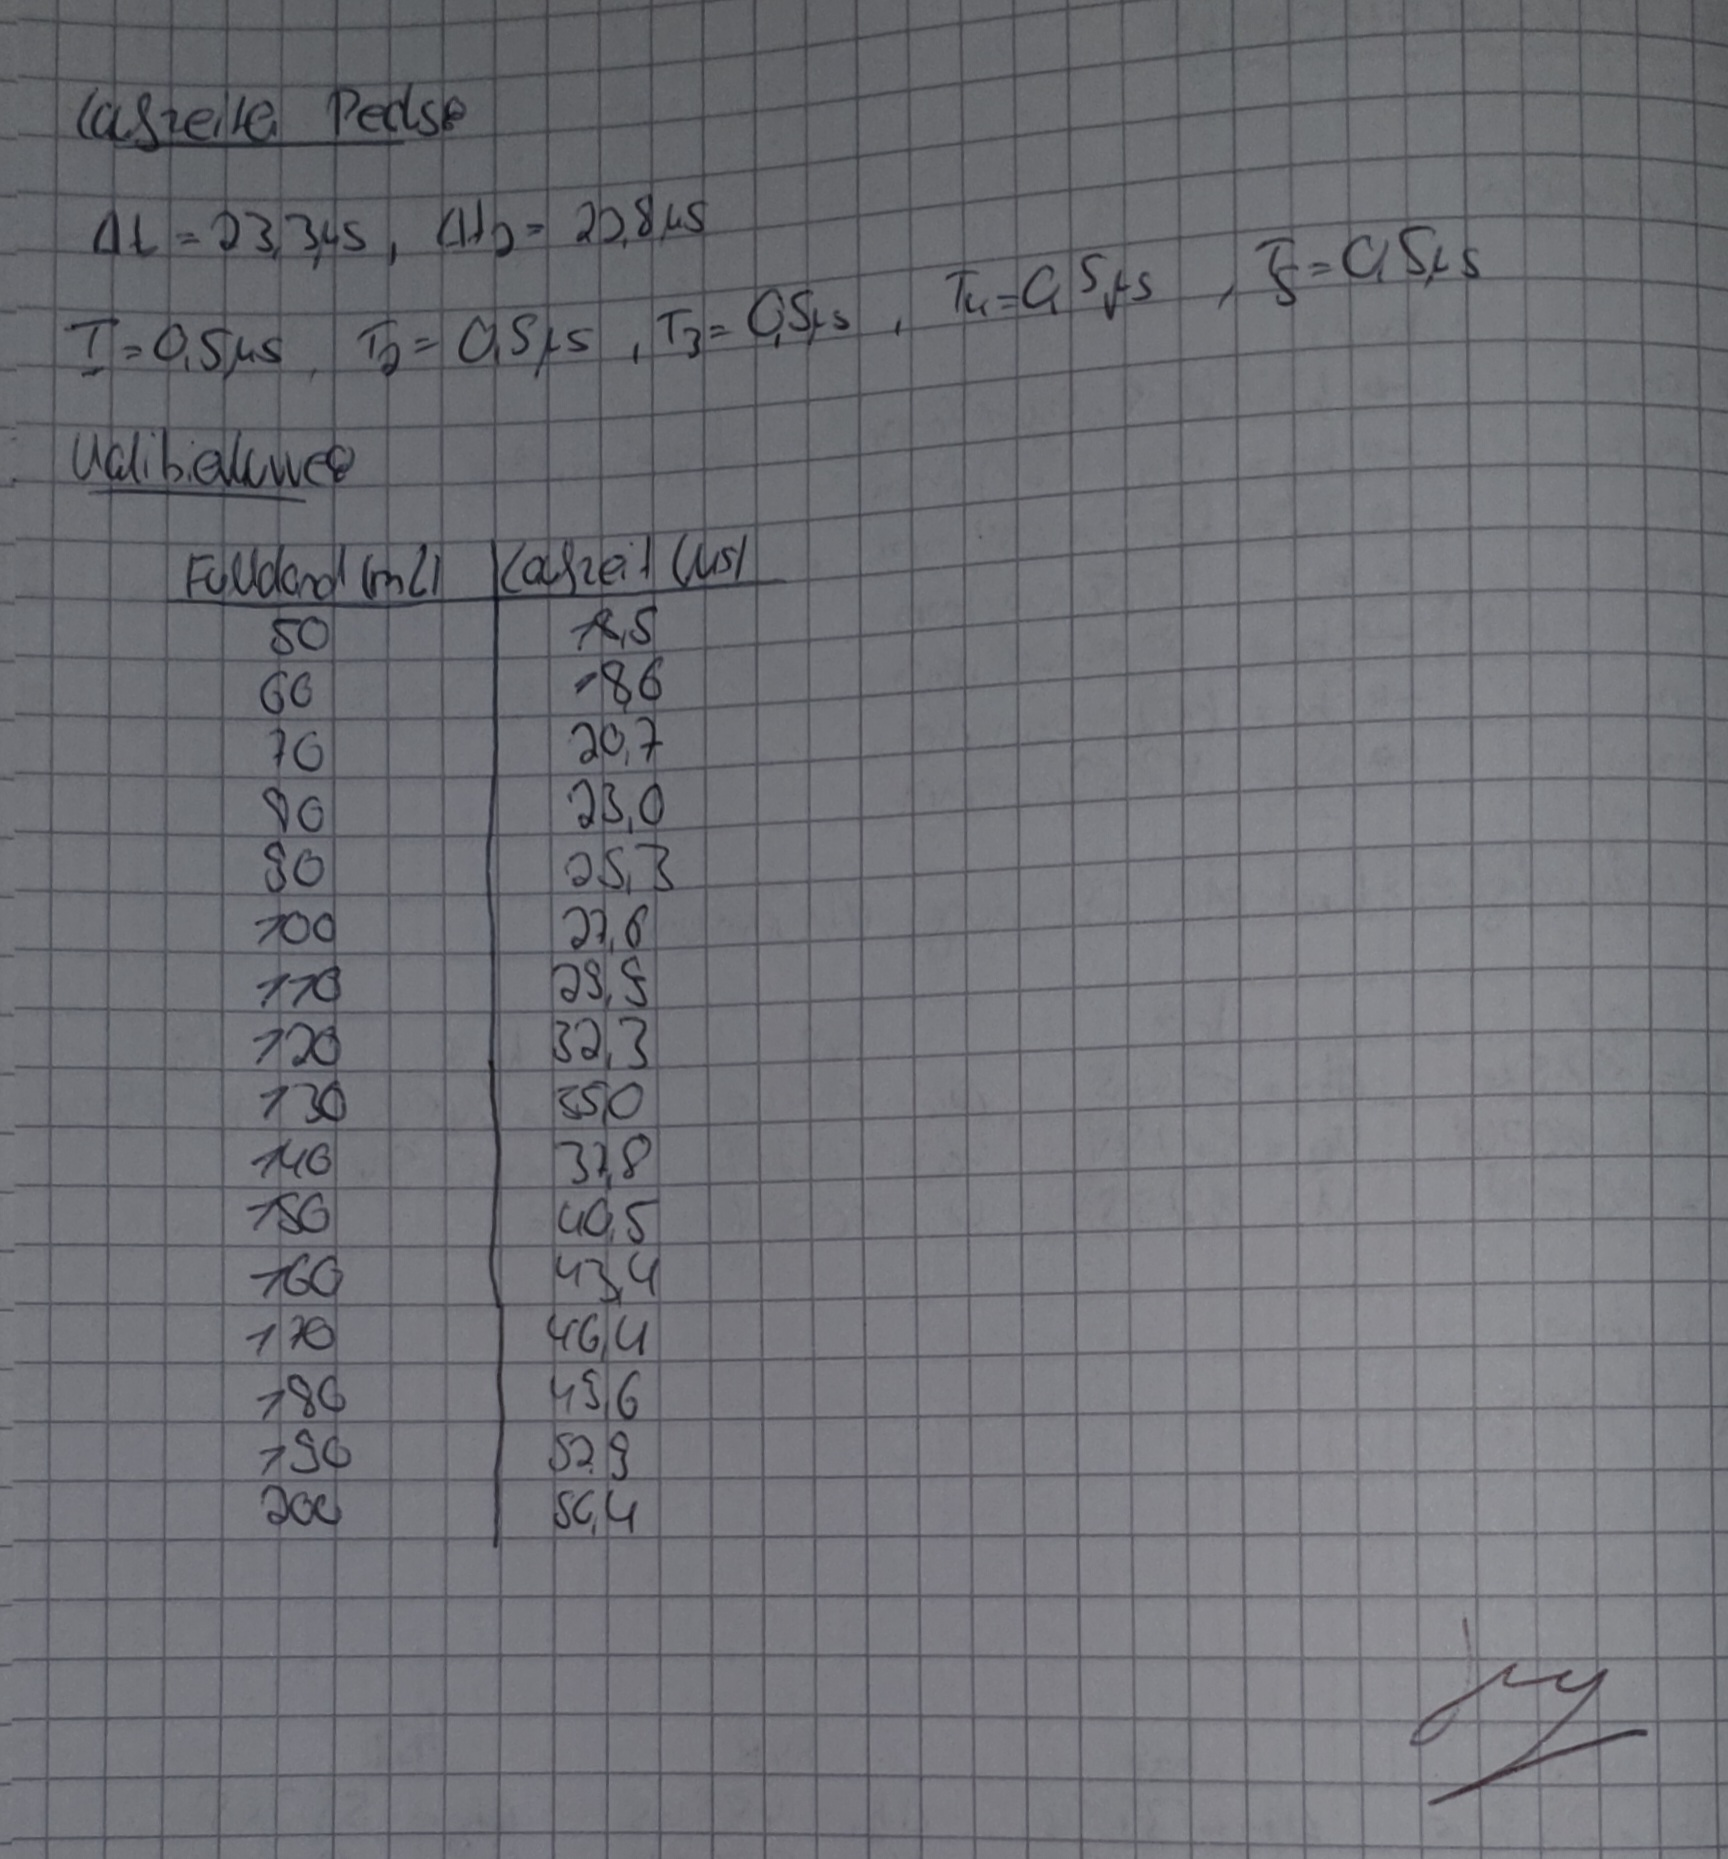
\includegraphics[width=0.9\textwidth]{Laborbuch2.jpg}
\end{figure}

%\end{document}
